\newpage
\section{Latch Etapa de búsqueda - Etapa de decodificaci\'on}
\subsection{M\'odulo}
Este latch se encarga de mantener el valor de la instrucci\'on y el contador de programa para despu\'es de un clock pasarlo a la siguiente etapa, la etapa de decodificaci\'on.

\begin{figure}[H]
\centering
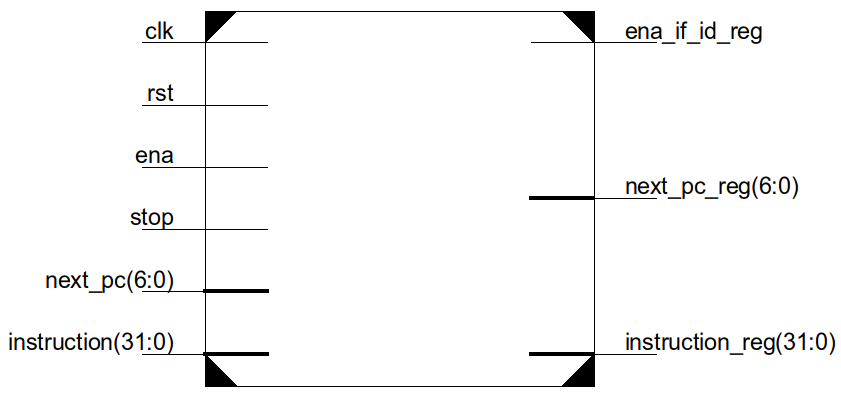
\includegraphics[scale=0.35]{img/latch_if_id}
\caption{Latch etapa de busqueda, etapa de decodificaci\'on}
\label{fig:latchifid}
\end{figure}

Como se puede ver en la figura \ref{fig:latchifid} el latch tiene las siguientes entradas:
\begin{itemize}
  \item \textbf{clk}: Clock que gobierna todo el sistema.
  \item \textbf{rst}: Entrada de reset.
  \item \textbf{ena}: Habilitaci\'on del chip.
  \item \textbf{stop}: A diferencia del ena, esta señal se encarga de retener la instruccion hasta que se d\'e de baja esta señal.
  \item \textbf{next\_pc}: Entrada del contador de programa. El prop\'osito es para utilizarlo en las pr\'oximas etapas por si existe una instrucci\'on de salto para sumarlo a este valor.
  \item \textbf{instruction}: Bus de datos que contiene el valor de la instrucci\'on a ejecutar.  
\end{itemize}

Las salidas de este m\'odulo son:
\begin{itemize}
  \item \textbf{ena\_if\_id\_reg}: Pasa a la etapa de decodificaci\'on la señal enable.
  \item \textbf{next\_pc\_reg}: Contador de programa de la etapa de b\'usqueda de la instrucci\'on.
  \item \textbf{instruction\_reg}: Instrucci\'on de la etapa de b\'usqueda.
\end{itemize}